\chapter{Conector y esquemas}
El conector KF2510 de siete pines está numerado en la placa. Use la orientación de la fotografía y los números, no solo los colores de los cables. Pin 1: K30/KL30, alimentación; pin 2: V2; pin 3: V1; pin 4: 1WRE, One-Wire; pin 5: KL, K-Line reservada; pin 6: salida +5 V, máximo 30 mA; pin 7: GND, masa.

El esquema del voltímetro identifica la K-Line reservada y el límite de corriente de +5 V. No se especifican límites generales para las entradas analógicas. La indicación de 12 V para Check Engine no implica que otras entradas admitan esa tensión. Utilice el esquema específico del sensor.

Las ilustraciones originales conservan sus etiquetas en inglés; este manual explica las funciones correspondientes.

\begin{figure}[H]
\centering
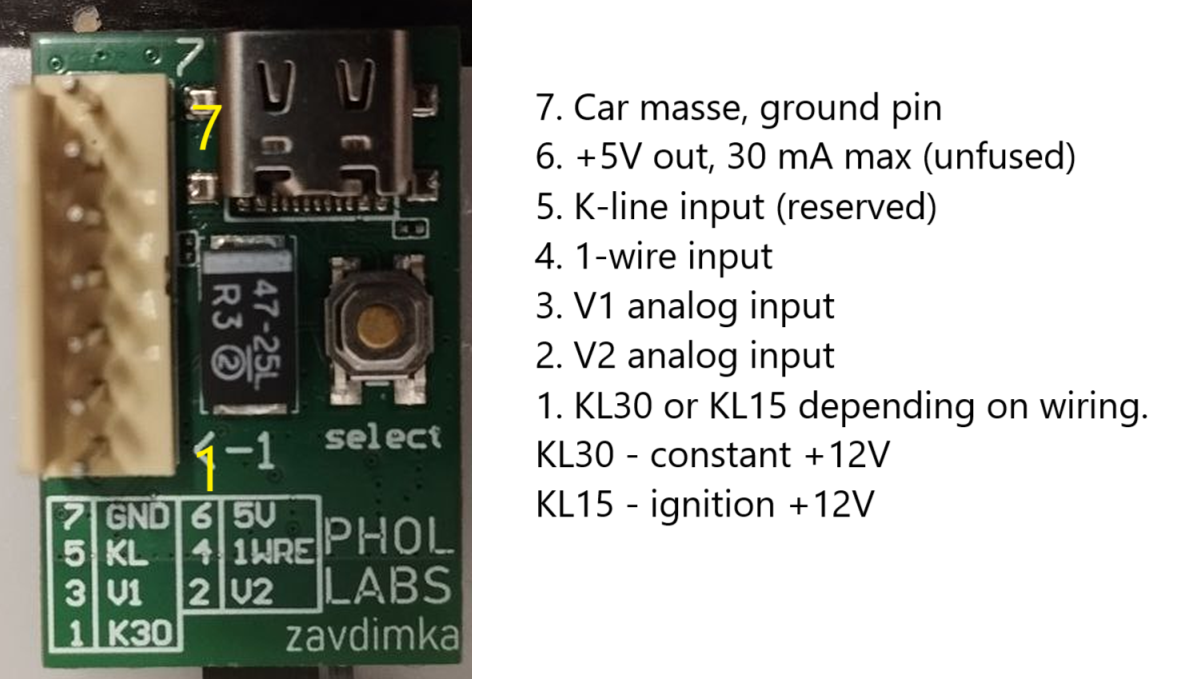
\includegraphics[width=.85\textwidth,height=.60\textheight,keepaspectratio]{figures/ivevo/image20.png}
\caption{Conector y esquemas}
\end{figure}
\clearpage
\section{Voltímetro}

\begin{figure}[H]
\centering
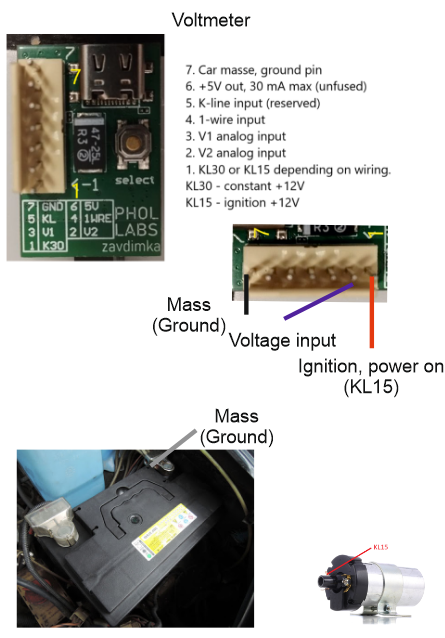
\includegraphics[width=.85\textwidth,height=.60\textheight,keepaspectratio]{figures/ivevo/image5.png}
\caption{Voltímetro}
\end{figure}
\clearpage
\section{Indicador de marcha}

\begin{figure}[H]
\centering
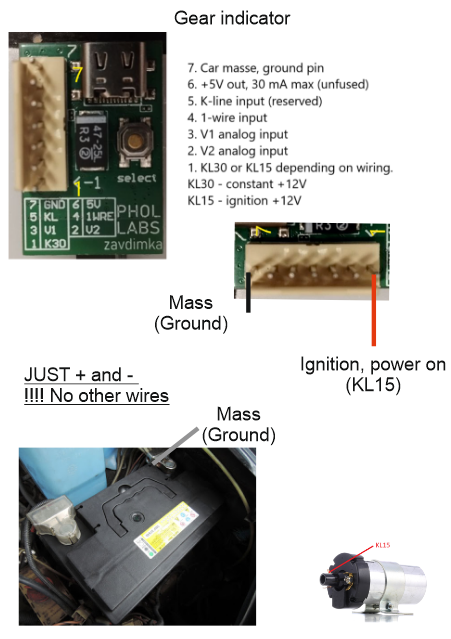
\includegraphics[width=.85\textwidth,height=.60\textheight,keepaspectratio]{figures/ivevo/image6.png}
\caption{Indicador de marcha}
\end{figure}
\clearpage
\section{Presión de aceite}

\begin{figure}[H]
\centering
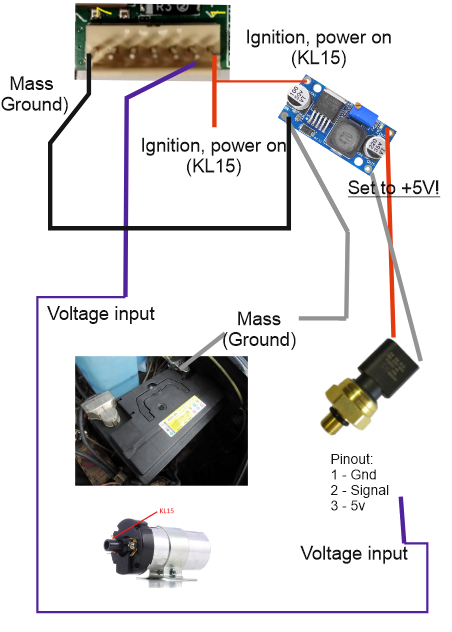
\includegraphics[width=.85\textwidth,height=.60\textheight,keepaspectratio]{figures/ivevo/image1.png}
\caption{Presión de aceite}
\end{figure}
\clearpage
\section{Termómetro NTC}

\begin{figure}[H]
\centering
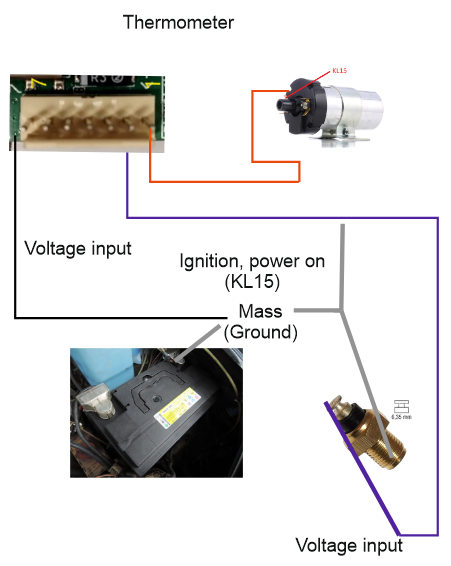
\includegraphics[width=.85\textwidth,height=.60\textheight,keepaspectratio]{figures/ivevo/image13.png}
\caption{Termómetro NTC}
\end{figure}
\clearpage
\section{Termómetro digital}

\begin{figure}[H]
\centering
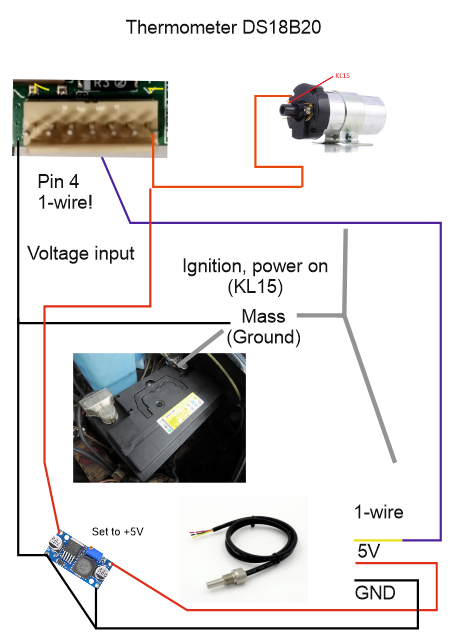
\includegraphics[width=.85\textwidth,height=.60\textheight,keepaspectratio]{figures/ivevo/image8.png}
\caption{Termómetro digital}
\end{figure}
\clearpage
\section{Lambda de banda ancha}

\begin{figure}[H]
\centering
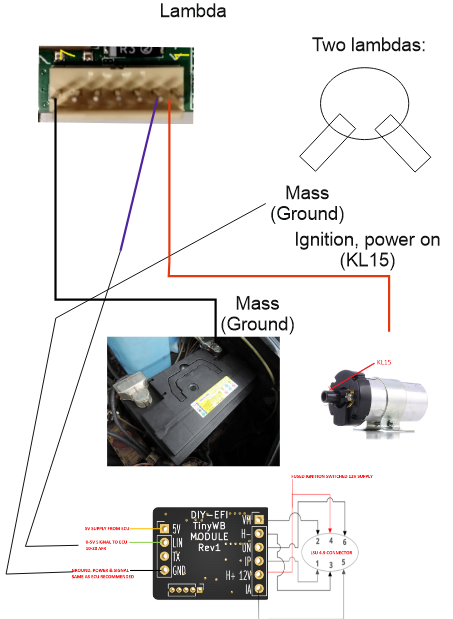
\includegraphics[width=.85\textwidth,height=.60\textheight,keepaspectratio]{figures/ivevo/image3.png}
\caption{Lambda de banda ancha}
\end{figure}
\clearpage
\section{Sobrealimentación}

\begin{figure}[H]
\centering
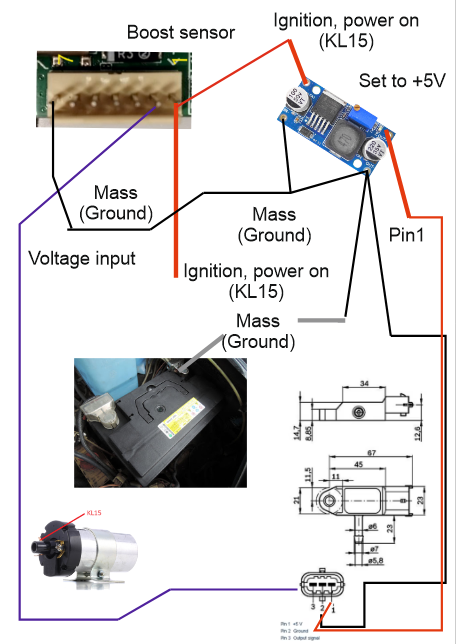
\includegraphics[width=.85\textwidth,height=.60\textheight,keepaspectratio]{figures/ivevo/image17.png}
\caption{Sobrealimentación}
\end{figure}
